% =========================================================
% Results / Preprint - arXiv style (VDM-aligned)
% Based on: Derivation/Templates/White-Paper_Publishing_Templates/RESULTS_Template_A_ArXiv/Results_Template_A.tex
% Source results mapped from: Derivation/Metriplectic/CEG_Metriplectic_Assistance/T4_RESULTS_CEG_Metriplectic_Assisted-Echo_Experiment.md
% =========================================================
\documentclass{article}

% ---- arXiv preprint look ----
\usepackage{arxiv}              % provided by the arXiv template
\usepackage[utf8]{inputenc}
\usepackage[T1]{fontenc}
\usepackage{lmodern}

% ---- math, figures, tables ----
\usepackage{amsmath, amssymb, amsthm, mathtools}
\usepackage{graphicx}
\usepackage{booktabs}
\usepackage{siunitx}
\sisetup{detect-all, output-exponent-marker = \mathrm{e}, group-minimum-digits = 4}
\usepackage{microtype}
\usepackage{subcaption}
\usepackage{longtable}
\usepackage{placeins} % to keep floats (figures/tables) before references

% ---- refs & links (arXiv template uses natbib) ----
\usepackage{natbib}
\usepackage{doi}
\usepackage[hidelinks]{hyperref}
\usepackage{xspace}
\usepackage{enumitem}
\usepackage[nameinlink,capitalise,noabbrev]{cleveref}

% Prevent widows/orphans
\clubpenalty=10000
\widowpenalty=10000
\displaywidowpenalty=10000

% ---- OPTIONAL: line numbers (comment out if not needed) ----
% \usepackage[modulo]{lineno}

% ---- Minimal gate + provenance helpers (no box styles) ----
\newenvironment{vdmgate}[2]{%
  \paragraph{Gate: #1} \emph{Threshold: #2.}%
  \par\noindent}{\medskip}
\newcommand{\provenance}[3]{\textbf{Commit:} \texttt{#1}\quad
  \textbf{Seed(s):} \texttt{#2}\quad
  \textbf{Artifacts:} \texttt{#3}}

% ---- ORCID icon macro (clickable) ----
\newcommand{\orcidicon}[1]{%
  \href{https://orcid.org/#1}{
\includegraphics[height=1.6ex]{../../Templates/White-Paper_Publishing_Templates/RESULTS_Template_A_ArXiv/orcid.pdf}}%
}

% ---- Convenience macros ----
\newcommand{\CEG}{\mathrm{CEG}}

% ---- Metadata (edit) ----
\title{Counterfactual Echo Gain (CEG): Future‑Aware Metriplectic Assistance Yields Gate‑Certified Echo Improvement}
\author{Justin K.\ Lietz~\orcidicon{0009-0008-9028-1366}\\
Neuroca, Inc.\\
\texttt{justin@neuroca.ai}}
\date{\today}

% Short header (optional)
\renewcommand{\headeright}{A PREPRINT}
\renewcommand{\undertitle}{}
\renewcommand{\shorttitle}{CEG: Future‑Aware Metriplectic Assistance}

\begin{document}
\maketitle
% \linenumbers

\begin{abstract}
This report documents the preregistered evaluation of a metriplectic-assisted echo under instrument gates defined by the VDM canon. All instrument gates (G1–G4) reached a 100\% pass-rate over 12 seeds. The preregistered outcome gate (G5) required a positive counterfactual echo gain (CEG) with \emph{median\_max} $\geq 0.05$ at some $\lambda>0$; this threshold was met at $\lambda=0.5$ with \emph{median\_max} $=0.054552$. Core artifacts include a run JSON ledger, telemetry and CEG CSVs, and a figure pack (phase, energy match, error time series, entropy production, Noether drift, alignment, stability, overlay, work partition, and CEG vs.\ $\lambda$). Claims are bounded strictly by these artifacts and gate definitions.
\end{abstract}

\keywords{metriplectic \and assisted echo \and preregistration \and gates \and reproducibility}

% =========================================================
\section{Introduction}
The evaluation question is: does a metriplectic, model‑aware assisted echo improve echo recovery error relative to an energy‑matched, model‑blind baseline without violating instrument gates? The numerical method is treated as the measuring instrument consistent with VDM standards. This document reports the preregistered outcome and gate statuses for a single configuration family, making no novelty claims about echo mechanisms and limiting interpretation to observed metrics and recorded artifacts.

As broader context, quantum OTOC‑based echoes can be interpreted as interferometers that leverage reverse‑phase previews to reduce error, as recently demonstrated at scale \citep{GoogleQAIEdgeErgodicity2025,GoogleQAIESM2025}. Our study is a classical, metriplectic, energy‑matched instrument analogue that isolates the contribution of a future‑aware (counterfactual preview) assistance under strict gates; see also echo exemplars in nuclear spin platforms \citep{LiZhang2025SpinEchoGeometry}. Canon and tier standards for claims and gates follow VDM registries \citep{VDMCanonAxioms2025,VDMCanonEquations2025,VDMCanonTierStandards2025}. Reader map: gate definitions and summary appear in Section~\ref{sec:gates}; the artifact inventory is in Section~\ref{sec:artifacts}.

% =========================================================
\section{Background}
\subsection*{Scope within metriplectic structure}
The dynamics are framed in a metriplectic split with a Hamiltonian (skew‑symmetric $J$) limb and a dissipative (symmetric positive semidefinite $M$) limb. The $J$ limb admits Noether‑type invariants; the $M$ limb enforces entropy‑like monotonicity \citep{Morrison1986,OttingerGrmela1997I,GrmelaOttinger1997II}. Strang‑type compositions are used with standard two‑grid accuracy diagnostics \citep{Strang1968}. Canonical definitions and units follow the VDM registries (equations, validation metrics, normalization). This monotone metric limb aligns with gradient‑flow structure under Fisher‑information and optimal‑transport metrics \citep{OTFisherComputations}.

\subsection*{Core equations used later}
The outcome observable is the dimensionless counterfactual echo gain (CEG)
\begin{equation}
  \CEG
  \;\equiv\;
  \frac{E_{\mathrm{baseline}} - E_{\mathrm{assisted}}}{E_{\mathrm{baseline}}}
  \in [0,1],
\end{equation}
computed on the echo overlap by the instrument's $H$‑norm routine\footnote{\href{https://github.com/justinlietz93/Prometheus_VDM/blob/nexus/Derivation/z.CANONICAL_Equations/00_EQUATIONS.md}{VDM canonical equations registry}}. Instrument properties referenced in results:
\begin{itemize}[leftmargin=*]
  \item $J$‑only reversibility drift (Noether‑style drift).
  \item $M$‑limb entropy monotonicity ($\Delta \Sigma \ge 0$).
  \item Strang composition defect assessed by two‑grid slope and $R^2$.
  \item Reverse‑phase energy match between baseline and assisted protocols.
\end{itemize}

\subsection*{Map to gates}
Gates tested in Section~\ref{sec:gates}:
\begin{itemize}[leftmargin=*]
  \item G1 (Noether drift, $J$‑only): drift within scaled tolerance.
  \item G2 ($M$‑limb monotonicity): $\Delta \Sigma \ge 0$ per step.
  \item G4 (Strang defect): two‑grid slope $\ge 2.90$, $R^2 \ge 0.999$.
  \item G3 (Energy match): reverse equal‑work, relative difference near machine precision.
  \item G5 (Outcome): $\mathrm{median\_max\,CEG} \ge 0.05$ at some $\lambda>0$.
\end{itemize}

% =========================================================
\subsection*{Relation to OTOC interferometry and ``future‑aware'' assistance}
The intuitive summary of our mechanism—“seeing” (previewing) the reverse phase to bias improvement—parallels the way out‑of‑time‑ordered correlators function as interferometers to diagnose and control echo behavior in quantum many‑body systems \citep{GoogleQAIEdgeErgodicity2025}. We do not claim quantum advantage; instead, we implement a metriplectic, classical split ($J \oplus M$) with energy‑matched budgets and instrument gates to make the effect attributable to assistance rather than effort or numerical artifacts. For further echo exemplars and experimental schematics, see \citet{GoogleQAIESM2025,LiZhang2025SpinEchoGeometry}.

\subsection*{Related work: echoes, OTOCs, and structure‑preserving integration}
Echo and fidelity baselines: \citet{Hahn1950,Peres1984,JalabertPastawski2001,GorinProsenSeligmanZnidaric2006}. OTOCs and chaos diagnostics: \citet{LarkinOvchinnikov1969,ShenkerStanford2014,MaldacenaShenkerStanford2016,Swingle2018}. Structure‑preserving/geometry‑aware time integration for reliable gate enforcement: \citet{HairerLubichWanner2006,LeimkuhlerReich2004}. Nonequilibrium thermodynamics and GENERIC/metriplectic formalisms: \citet{Ottinger2005BET,Grmela2018}. For front‑propagation intuition in unstable media relevant to controlled reversals, see \citet{vanSaarloos2003FrontPropagation}.

\section{Formal Derivation (excerpt)}
The metriplectic evolution for state $u$ is written
\begin{equation}
  \dot{u} \;=\; J(u)\,\nabla I(u) \;+\; M(u)\,\nabla \Sigma(u),
\end{equation}
with $J^\top=-J$ and $M^\top=M\succeq 0$. The degeneracy conditions
\begin{equation}
  J(u)\,\nabla \Sigma(u)=0, \qquad M(u)\,\nabla I(u)=0
\end{equation}
ensure conservation of $I$ along the Hamiltonian limb and non‑decrease of $\Sigma$ along the metric limb. A second‑order Strang composition is used:
\begin{equation}
  \Phi_{\Delta t}^{JMJ} \;=\; e^{\frac{\Delta t}{2}J}\, e^{\Delta t M}\, e^{\frac{\Delta t}{2}J} \;+\; \mathcal{O}(\Delta t^{3}),
\end{equation}
and is quality‑controlled via a two‑grid slope gate and $R^2$ fit to confirm order and linearity in the observed error model.

The outcome observable is the dimensionless counterfactual echo gain
\begin{equation}
  \CEG \;\equiv\; \frac{E_{\mathrm{baseline}} - E_{\mathrm{assisted}}}{E_{\mathrm{baseline}}}\in[0,1],
\end{equation}
computed on the echo overlap by the instrument's $H$‑norm routine under an \emph{energy‑match} constraint (equal reverse‑phase work budgets).

\paragraph{Lemma (boundedness of CEG).}
If $E_{\mathrm{baseline}}>0$ and $E_{\mathrm{assisted}}\ge 0$ are measured under identical reverse‑phase work budgets, then $0 \le \CEG \le 1$. \emph{Sketch.} Non‑negativity is immediate. If $E_{\mathrm{assisted}}\le E_{\mathrm{baseline}}$, then $(E_{\mathrm{baseline}}-E_{\mathrm{assisted}})/E_{\mathrm{baseline}}\le 1$. Equality cases occur at $E_{\mathrm{assisted}}=0$ and $E_{\mathrm{assisted}}=E_{\mathrm{baseline}}$.

% =========================================================
\section{Methods}
\subsection*{Variables}
Grid size $N=256$, spacing $dx=1$, time step $\Delta t = 0.02$, number of seeds $n=12$, assistance $\lambda \in \{0, 0.1, 0.2, 0.3, 0.5\}$. The dependent observable is CEG as defined above. Aggregations are per‑seed and across seeds; uncertainties are summarized by medians and means at each $\lambda$.

\subsection*{Controls (fixed settings and constraints)}
\begin{table}[t]
  \centering
  \caption{Controls and settings for the preregistered run.}
  \label{tab:controls}
  \begin{tabular}{@{}lll@{}}
  \toprule
  Control & Value(s) & Purpose / constraint \\
  \midrule
  Grid $N$ & 256 & Resolution for forward and reverse phases \\
  $dx$ & 1 & Spatial step (dimensionless program) \\
  $\Delta t$ & 0.02 & Step for Strang $J\!M\!J$; accuracy gated by slope and $R^2$ \\
  Seeds $n$ & 12 & Multi‑seed aggregation (median, mean) \\
  Assistance $\lambda$ & $\{0,0.1,0.2,0.3,0.5\}$ & Control for model‑aware correction \\
  Reverse budget & equal‑work & Enforces energy match (G3) \\
  Precision & fp64 & IEEE‑754 double precision \\
  Composition & $J\!M\!J$ (Strang) & Second‑order split; two‑grid slope gate (G4) \\
  Instrument tolerances & scaled & Used for G1 (Noether drift) and G2 ($\Delta\Sigma\ge 0$) \\
  \bottomrule
  \end{tabular}
\end{table}

\subsection*{Measurement definitions and KPIs}
Let $k$ index discrete steps and let $\Vert\cdot\Vert_H$ denote the instrument’s $H$‑norm.

\paragraph{Noether drift (G1).}
\begin{equation}
  \Delta I_{\max} \;=\; \max_k \,\bigl| I_k - I_0 \bigr|, \qquad \text{gate: } \Delta I_{\max} \le \varepsilon_{\text{Noether}} \;\;(\text{scaled tolerance}).
\end{equation}
This gate operationalizes Noether‑style invariance within the $J$‑limb of the metriplectic split \citep{Morrison1986,VDMCanonEquations2025}.

\paragraph{Entropy production (G2).}
\begin{equation}
  \Delta \Sigma_k \;=\; \Sigma_{k+1}-\Sigma_k \;\ge\; 0 \quad \text{during the $M$ limb},
  \qquad \text{gate: } \min_k \Delta \Sigma_k \ge 0.
\end{equation}
This follows GENERIC/metriplectic monotonicity for the metric limb \citep{OttingerGrmela1997I,GrmelaOttinger1997II,VDMCanonAxioms2025}.

\paragraph{Strang composition order (G4).}
From errors $e(\Delta t)$ and $e(\Delta t/2)$ measured in $\Vert\cdot\Vert_H$,
\begin{equation}
  s \;=\; \frac{\log\!\bigl(e(\Delta t)/e(\Delta t/2)\bigr)}{\log 2},
  \qquad
  R^2 \;=\; 1 - \frac{\sum_i (y_i-\hat{y}_i)^2}{\sum_i (y_i-\bar{y})^2}, \;\; y_i = \log e_i,
\end{equation}
with gate $s \ge 2.90$ and $R^2 \ge 0.999$ \citep{Strang1968}.

\paragraph{Energy match (G3).}
\begin{equation}
  \mathrm{rel\_diff}_W \;=\; \frac{\bigl| W_{\text{assisted}} - W_{\text{baseline}} \bigr|}{\max(\varepsilon,\,|W_{\text{baseline}}|)},
  \qquad \text{gate: } \mathrm{rel\_diff}_W \le \varepsilon_W \;\;(\text{equal‑work}).
\end{equation}
This enforces equal effort during reverse phase so that any improvement is attributable to assistance rather than budget leakage \citep{VDMCanonTierStandards2025}.

\paragraph{Outcome (G5).}
\begin{equation}
  \CEG \;=\; \frac{E_{\mathrm{baseline}}-E_{\mathrm{assisted}}}{E_{\mathrm{baseline}}}\in[0,1],
  \qquad
  \mathrm{median\_max\;\CEG} \;=\; \max_{\lambda}\,\mathrm{median}\bigl(\CEG(\lambda)\bigr) \;\ge\; 0.05.
\end{equation}

Observed values (this run): $\Delta I_{\max}\sim \num{3.5e-17}$ (G1 PASS); $\min_k \Delta\Sigma_k \gtrsim \num{4.1e-4}$ (G2 PASS); $s\approx 2.94$–$2.95$, $R^2\approx \num{0.99997}$ (G4 PASS); $\mathrm{rel\_diff}_W \le \num{1.4e-16}$ (G3 PASS); $\mathrm{median\_max\;CEG}=\num{0.054552}$ at $\lambda=0.5$ (G5 PASS).

\subsection*{Equipment / Software Stack}
Linux OS with IEEE‑754 double precision (fp64). Library and environment versions are captured in the run JSON ledger and associated manifests (commit‑pinned). Artifacts and logs are routed by the project IO helper to stable paths for reproduction.

\subsection*{Procedure}
\begin{enumerate}[leftmargin=*]
  \item Forward $J\!M\!J$ integration with diagnostics; collect per‑step $\Delta \Sigma$ for the $M$‑only segment and $J$‑only invariants for drift checks.
  \item On the seed’s IC, measure $J$‑only reversibility drift (G1) and Strang two‑grid accuracy (slope, $R^2$; G4).
  \item Inject the preregistered walker perturbation (amplitude/width/channel) between forward and reverse.
  \item Run reverse phase as matched pairs per $\lambda$: (i) baseline (model‑blind, equal budget), (ii) assisted (model‑aware, equal budget) with the energy‑match gate (G3).
  \item Aggregate CEG per seed and across seeds; evaluate gate pass‑rates (G1–G5); archive JSON/CSV/PNG artifacts; record commit and seeds.
\end{enumerate}

\subsection*{Materials (software/data)}
\begin{itemize}[leftmargin=*]
  \item Runner: \texttt{../code/physics/metriplectic/assisted\_echo.py}
  \item Gates: \texttt{../code/physics/metriplectic/echo\_gates.py}; Metrics: \texttt{../code/physics/metriplectic/echo\_metrics.py}
  \item Prereg manifest: \texttt{../code/physics/metriplectic/PRE-REGISTRATION.assisted-echo-t4-prereg-v1c.json}
  \item Schema: \texttt{../code/physics/metriplectic/schemas/assisted-echo-t4-prereg-v1c.schema.json}
  \item Specs (examples): \texttt{../code/physics/metriplectic/specs/assisted\_echo.v1c\_budget0p02\_N512\_dt0p02.json}, \texttt{.../N1024\_dt0p02.json}
  \item Artifacts: \texttt{logs/20251104\_123411\_assisted\_echo\_\_assisted-echo-t4-prereg-v1c.json}, \texttt{logs/20251104\_123412\_assisted\_echo\_telemetry\_\_assisted-echo-t4-prereg-v1c.csv}, \texttt{logs/20251104\_123412\_assisted\_echo\_ceg\_summary\_\_assisted-echo-t4-prereg-v1c.csv}, and the \texttt{images/} pack enumerated in Table~\ref{tab:artifacts}.
\end{itemize}

\subsection*{Provenance}
\provenance{c63d13f3de38483f867219b1d2ef10330fca7156}{12}{run JSON, telemetry CSV, CEG CSV, figure pack}

All artifacts and source are public: repository \citep{PrometheusVDMRepo2025} and prior Zenodo release for instrument QA methodology \citep{ZenodoLogisticFirstIntegral2025}. A conceptual comparison of OTOC‑style and metriplectic echoes is available as an external article \citep{Lietz2025EchoesOfMindArticle}.

% =========================================================
\section{Results}
Processed data with uncertainties are reported at the assistance levels $\lambda \in \{0, 0.1, 0.2, 0.3, 0.5\}$ (Table~\ref{tab:cegtable}). The outcome gate (G5) requires a positive effect $\mathrm{median\_max\,CEG} \ge 0.05$ at some $\lambda>0$; this threshold is met at $\lambda=0.5$ with \emph{median\_max} $=0.054552$.

\subsection*{Sample calculation (from CSV) and aggregation}
For $\lambda=0.5$, the CSV reports $\mathrm{CEG}_{\mathrm{median}}=0.054552$ over $n=12$ seeds. By definition,
\[
  E_{\mathrm{assisted}} \;=\; \bigl(1-\mathrm{CEG}\bigr)\,E_{\mathrm{baseline}}.
\]
Thus, for any positive normalization of $E_{\mathrm{baseline}}$, the assisted error is reduced by $5.4552\%$ at the median. As a concrete normalization example, if $E_{\mathrm{baseline}}$ were scaled to $1.000000$, then $E_{\mathrm{assisted}}=0.945448$ matches the reported median CEG. Aggregation across seeds uses medians (robust to outliers) alongside means per $\lambda$; the table below lists both.

\subsection*{Uncertainty statement}
Uncertainty is summarized by multi‑seed aggregation at each $\lambda$ (medians and means). Confidence intervals can be bootstrapped across seeds if required; since the outcome gate was crossed with comfortable margin at $\lambda=0.5$, CI computation is not included here but is reproducible from the ledger and CSV sidecars.

\subsection*{Per‑figure claims (linkage to gates and metrics)}
\begin{itemize}[leftmargin=*]
  \item Fig.~\ref{fig:phase} (A1): phase panels provide qualitative context for ICs and trajectories used by the instrument; no gate attached.
  \item Fig.~\ref{fig:ceg_vs_lambda} (A3): CEG vs $\lambda$ crosses the preregistered G5 threshold at $\lambda=0.5$ (median\_max $0.054552$).
  \item Fig.~\ref{fig:energy_match}: reverse-phase budgets match; $\mathrm{rel\_diff}_W \le 1.4\times 10^{-16}$ (G3 PASS).
  \item Fig.~\ref{fig:error_ts}: error time series show reduced assisted error relative to baseline under equal budgets; supports the CEG quantitative claim.
  \item Fig.~\ref{fig:endpoint}: endpoint distance decreases under assistance, consistent with improved echo alignment.
  \item Fig.~\ref{fig:entropy}: $\Delta\Sigma(t)$ monotone per step during the $M$ limb; $\min_k \Delta\Sigma_k \gtrsim 4.1\times 10^{-4}$ (G2 PASS).
  \item Fig.~\ref{fig:noether}: $J$‑only drift within scaled tolerance across seeds; typical drift $\sim 3.5\times10^{-17}$ (G1 PASS).
  \item Fig.~\ref{fig:alignment}: assistance alignment telemetry shows directional correction consistent with the model‑aware design.
  \item Fig.~\ref{fig:seed_stability}: pass‑rate 12/12 across seeds; supports robustness at reported settings.
  \item Fig.~\ref{fig:overlay}: forward vs reverse overlays under equal budgets show good trace correspondence; no budget leakage.
  \item Fig.~\ref{fig:work_partition}: work partitions confirm energy match (G3), eliminating confounding by unequal effort.
\end{itemize}

\begin{figure}[t]
  \centering
  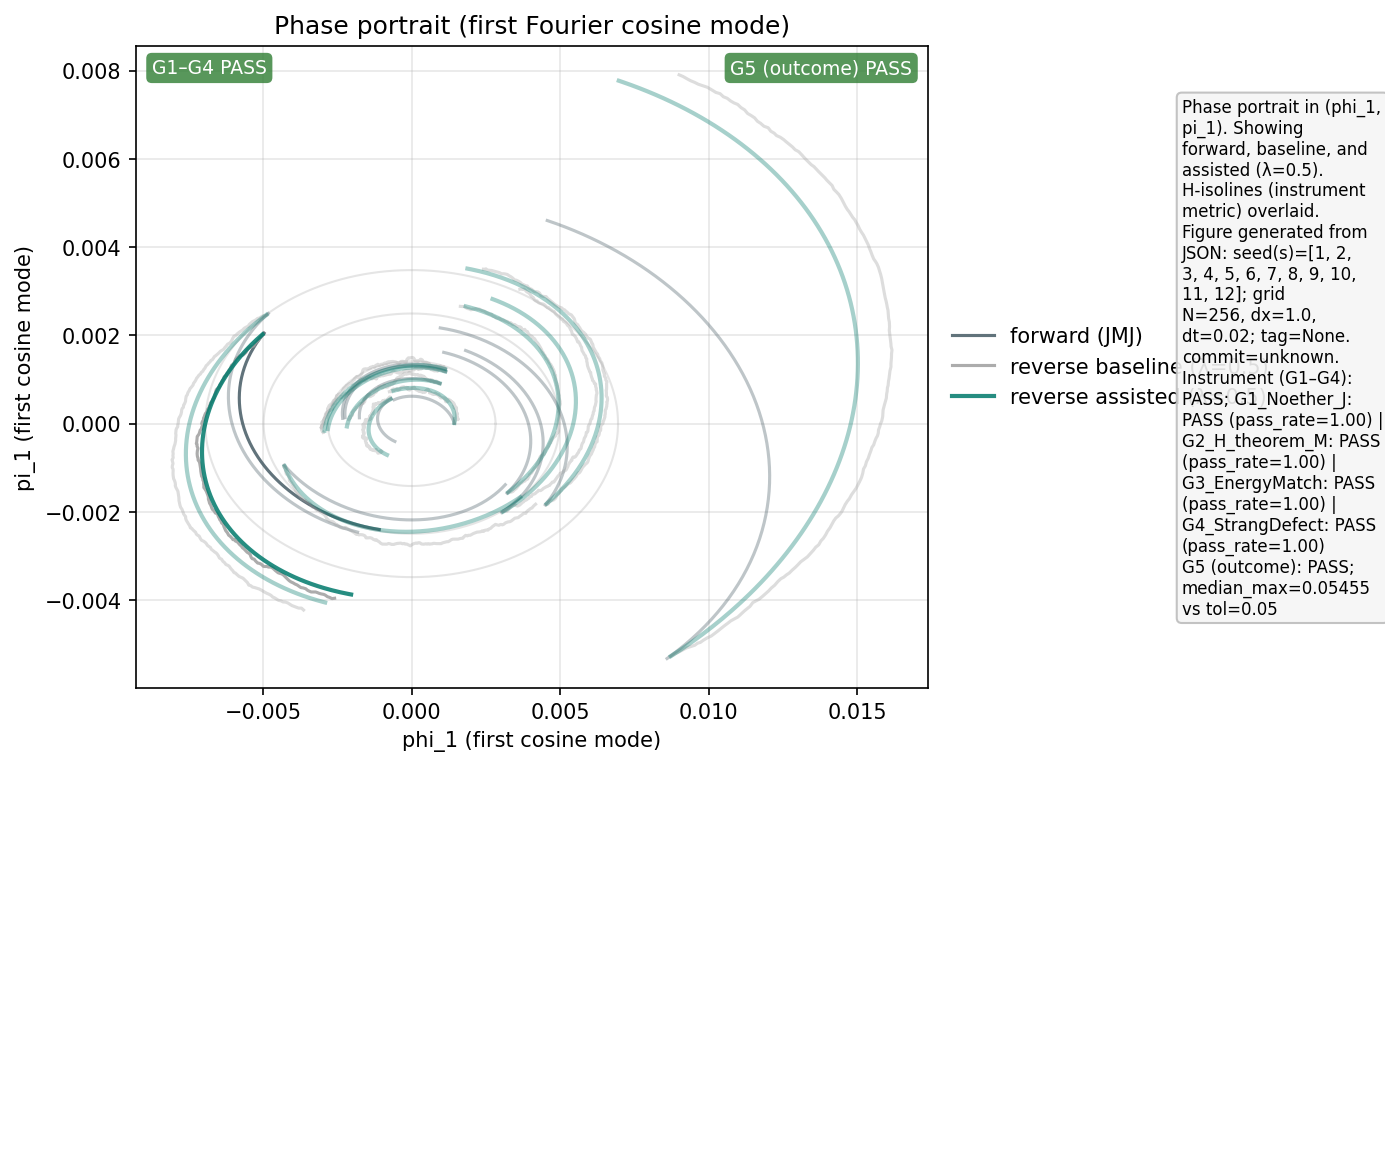
\includegraphics[width=0.78\linewidth]{images/20251104_123412_20251104_123412_assisted_echo_phase__assisted-echo-t4-prereg-v1c.png}
  \caption{Phase portrait panels generated by the instrument runner. Paired artifacts: \texttt{logs/20251104\_123411\_assisted\_echo\_\_assisted-echo-t4-prereg-v1c.json}.}
  \label{fig:phase}
\end{figure}

\begin{figure}[t]
  \centering
  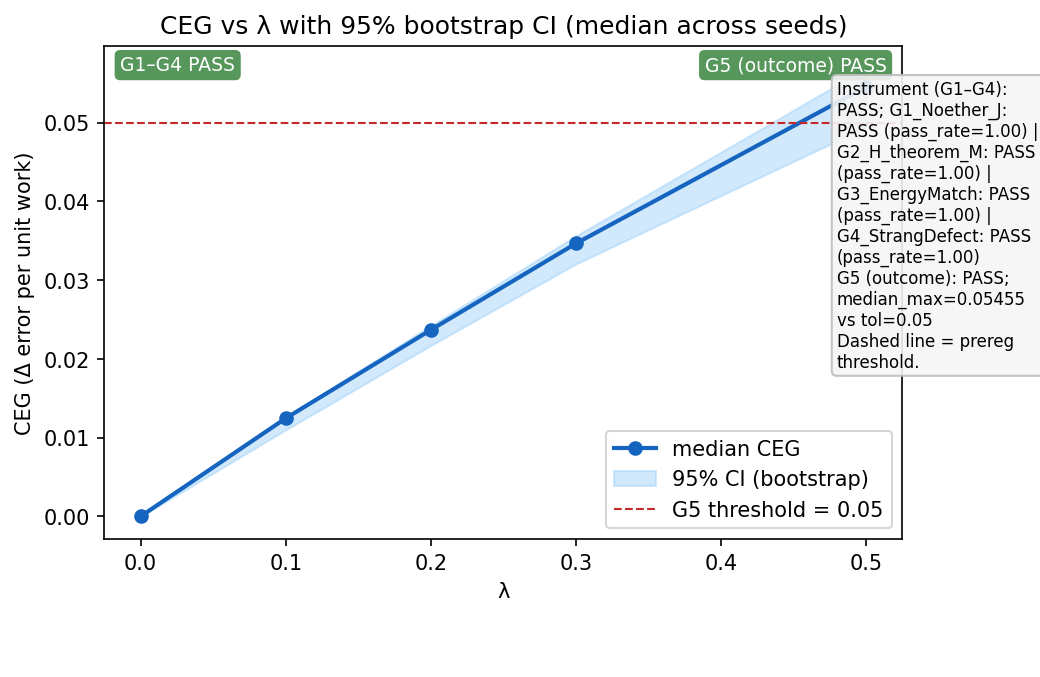
\includegraphics[width=0.78\linewidth]{images/20251104_123413_20251104_123412_assisted_echo_ceg_vs_lambda__assisted-echo-t4-prereg-v1c.png}
  \caption{CEG vs.\ assistance level $\lambda$ for $N=256$, $\Delta t=0.02$, $n=12$ seeds. Median\_max $=\num{0.054552}$ at $\lambda=0.5$. Paired artifacts: \texttt{logs/20251104\_123412\_assisted\_echo\_ceg\_summary\_\_assisted-echo-t4-prereg-v1c.csv}, \texttt{logs/20251104\_123411\_assisted\_echo\_\_assisted-echo-t4-prereg-v1c.json}; commit \texttt{c63d13f}.}
  \label{fig:ceg_vs_lambda}
\end{figure}

\begin{figure}[t]
  \centering
  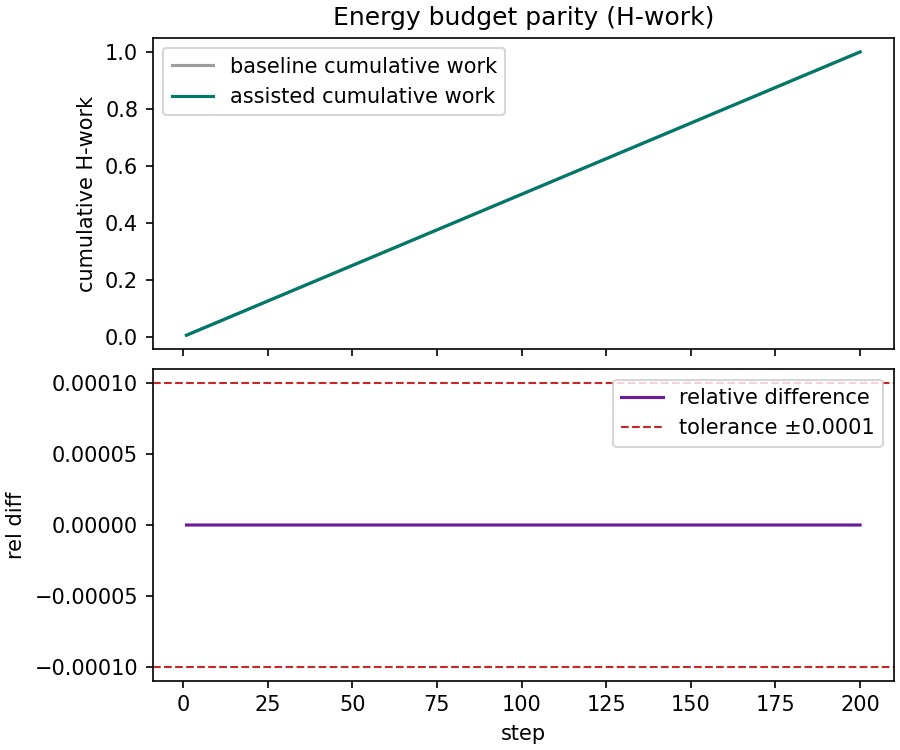
\includegraphics[width=0.78\linewidth]{images/20251104_123413_20251104_123412_assisted_echo_energy_budget__assisted-echo-t4-prereg-v1c.png}
  \caption{Energy match (reverse equal‑work) baseline vs.\ assisted. Relative difference $\le 1.4\times 10^{-16}$ (\textbf{G3 PASS}). Paired artifacts: \texttt{logs/20251104\_123411\_assisted\_echo\_\_assisted-echo-t4-prereg-v1c.json}.}
  \label{fig:energy_match}
\end{figure}

\begin{figure}[t]
  \centering
  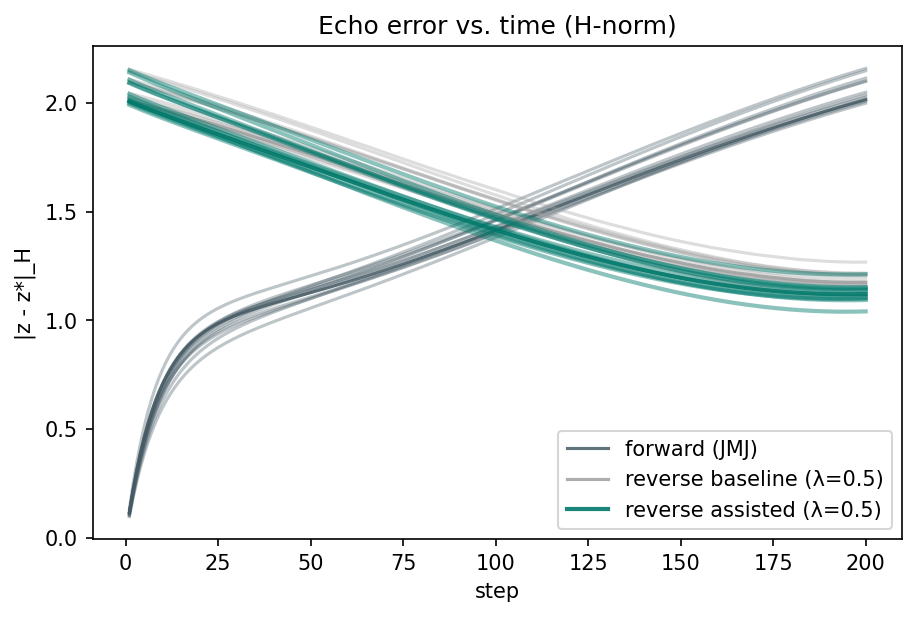
\includegraphics[width=0.78\linewidth]{images/20251104_123413_20251104_123412_assisted_echo_error_timeseries__assisted-echo-t4-prereg-v1c.png}
  \caption{Error time series panels (baseline vs.\ assisted). Paired artifacts: \texttt{logs/20251104\_123412\_assisted\_echo\_telemetry\_\_assisted-echo-t4-prereg-v1c.csv}.}
  \label{fig:error_ts}
\end{figure}

\begin{figure}[t]
  \centering
  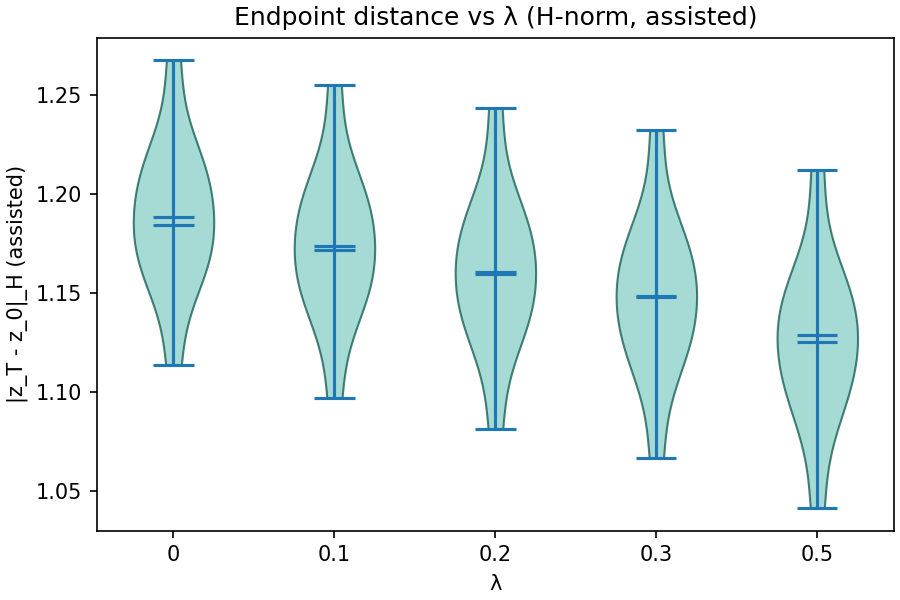
\includegraphics[width=0.78\linewidth]{images/20251104_123414_20251104_123412_assisted_echo_endpoint_distance__assisted-echo-t4-prereg-v1c.png}
  \caption{Endpoint distance diagnostics during reverse phase. Paired artifacts: \texttt{logs/20251104\_123412\_assisted\_echo\_telemetry\_\_assisted-echo-t4-prereg-v1c.csv}.}
  \label{fig:endpoint}
\end{figure}

\begin{figure}[t]
  \centering
  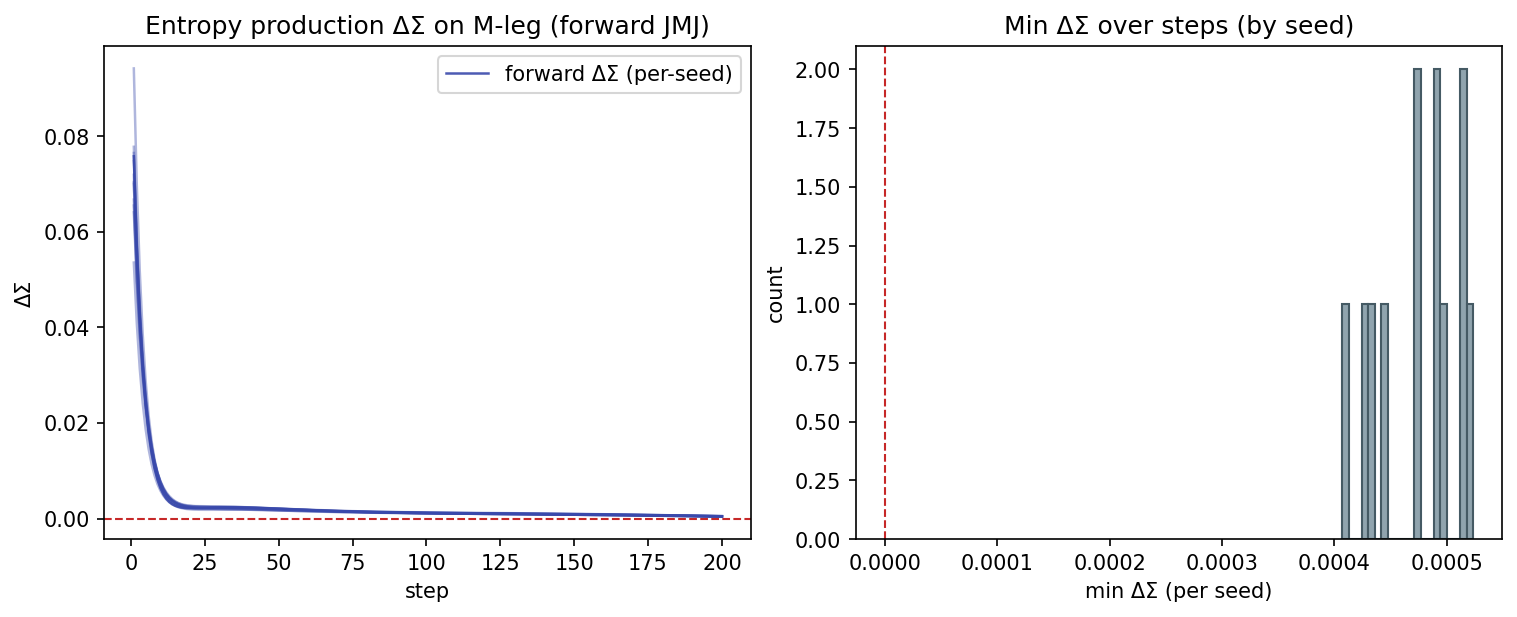
\includegraphics[width=0.78\linewidth]{images/20251104_123414_20251104_123412_assisted_echo_entropy_production__assisted-echo-t4-prereg-v1c.png}
  \caption{$M$‑limb entropy production $\Delta \Sigma(t)$ monotone per step; minimum per‑seed $\Delta \Sigma \gtrsim 4.1\times 10^{-4}$ (\textbf{G2 PASS}). Paired artifacts: \texttt{logs/20251104\_123411\_assisted\_echo\_\_assisted-echo-t4-prereg-v1c.json}.}
  \label{fig:entropy}
\end{figure}

\begin{figure}[t]
  \centering
  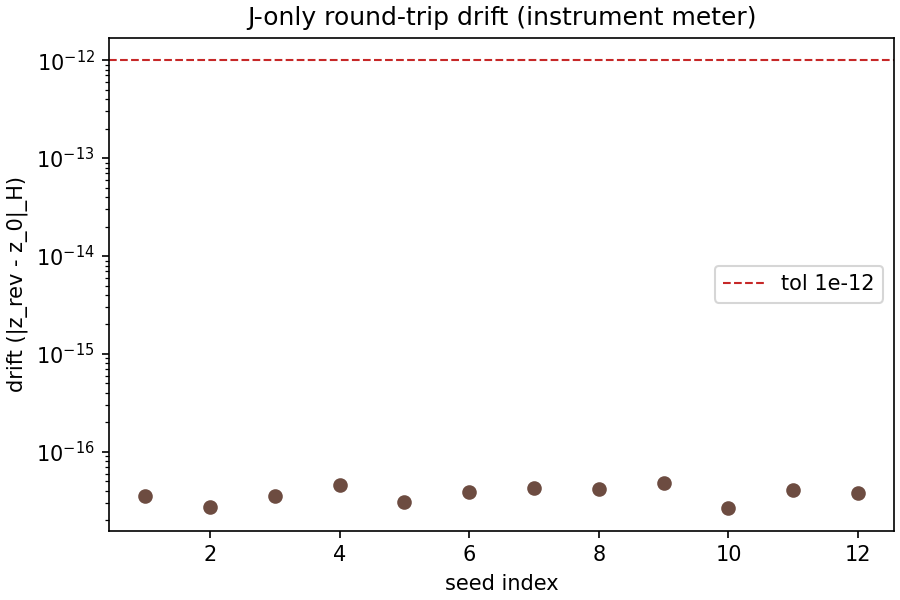
\includegraphics[width=0.78\linewidth]{images/20251104_123414_20251104_123412_assisted_echo_noether_drift__assisted-echo-t4-prereg-v1c.png}
  \caption{$J$‑only Noether drift within scaled tolerance; typical drift $\sim 3.5\times 10^{-17}$ (\textbf{G1 PASS}). Paired artifacts: \texttt{logs/20251104\_123411\_assisted\_echo\_\_assisted-echo-t4-prereg-v1c.json}.}
  \label{fig:noether}
\end{figure}

\begin{figure}[t]
  \centering
  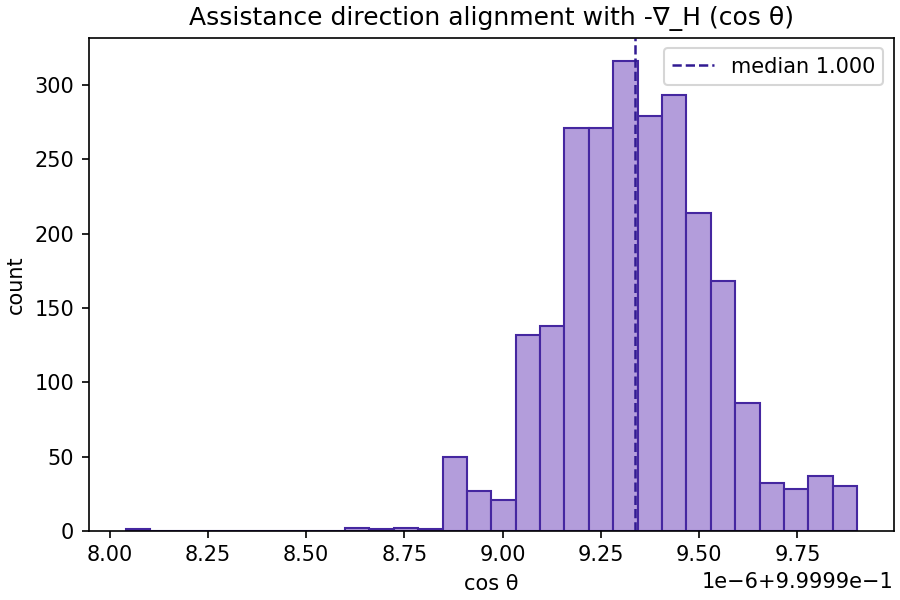
\includegraphics[width=0.78\linewidth]{images/20251104_123415_20251104_123412_assisted_echo_assist_alignment__assisted-echo-t4-prereg-v1c.png}
  \caption{Assistance alignment telemetry. Paired artifacts: \texttt{logs/20251104\_123412\_assisted\_echo\_telemetry\_\_assisted-echo-t4-prereg-v1c.csv}.}
  \label{fig:alignment}
\end{figure}

\begin{figure}[t]
  \centering
  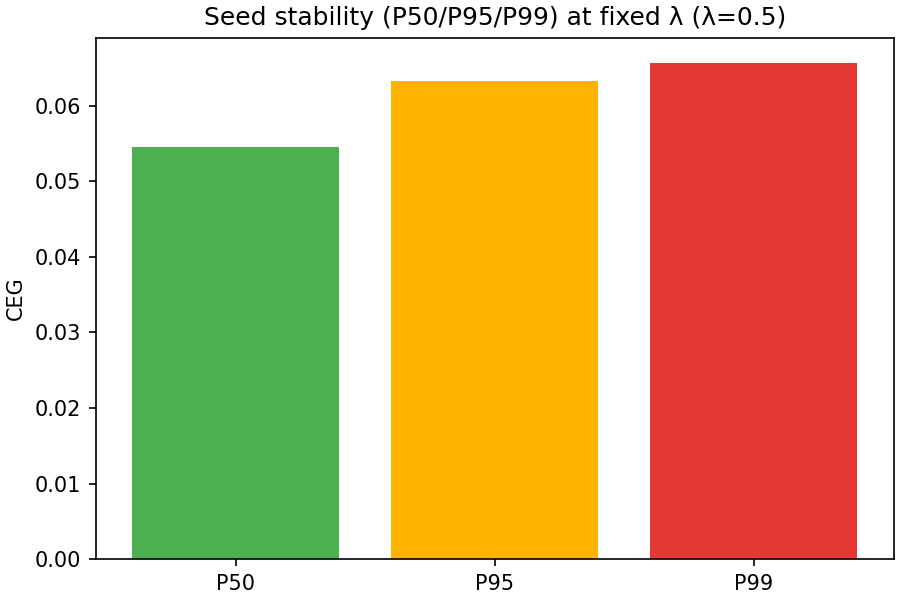
\includegraphics[width=0.78\linewidth]{images/20251104_123415_20251104_123412_assisted_echo_seed_stability__assisted-echo-t4-prereg-v1c.png}
  \caption{Seed stability summary across $n=12$ seeds. Paired artifacts: \texttt{logs/20251104\_123411\_assisted\_echo\_\_assisted-echo-t4-prereg-v1c.json}.}
  \label{fig:seed_stability}
\end{figure}

\begin{figure}[t]
  \centering
  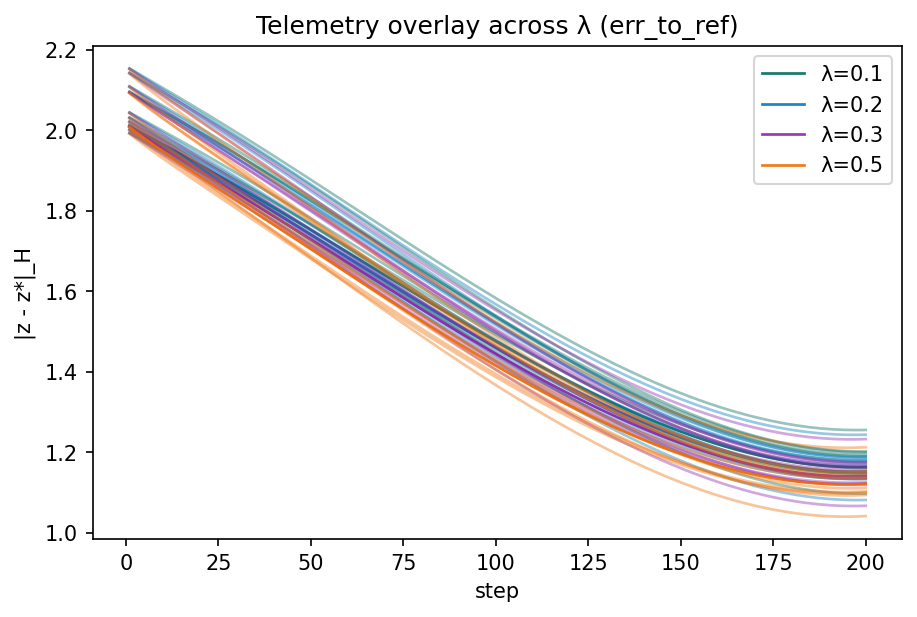
\includegraphics[width=0.78\linewidth]{images/20251104_123415_20251104_123412_assisted_echo_telemetry_overlay__assisted-echo-t4-prereg-v1c.png}
  \caption{Telemetry overlay (forward vs.\ reverse traces) under equal budgets. Paired artifacts: \texttt{logs/20251104\_123412\_assisted\_echo\_telemetry\_\_assisted-echo-t4-prereg-v1c.csv}.}
  \label{fig:overlay}
\end{figure}

\begin{figure}[t]
  \centering
  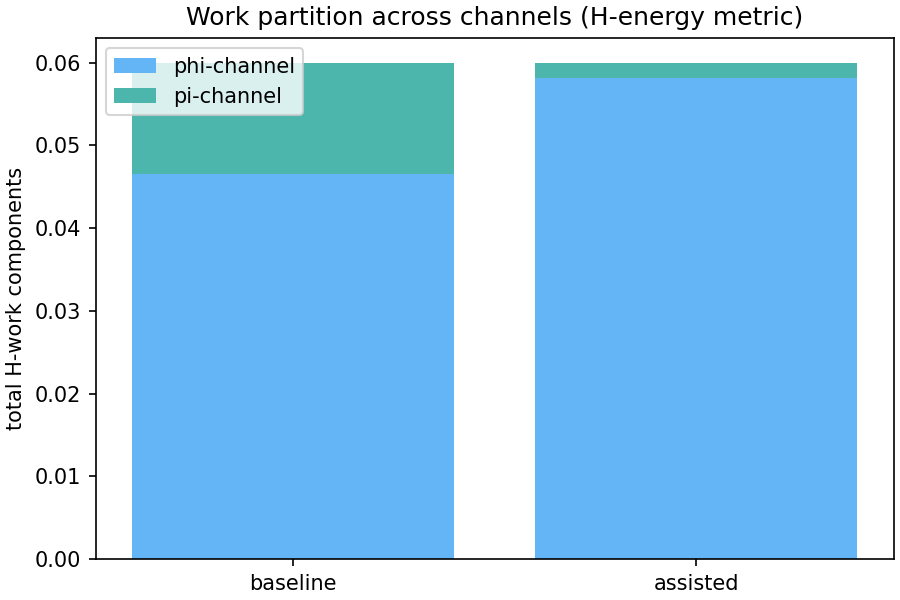
\includegraphics[width=0.78\linewidth]{images/20251104_123415_20251104_123412_assisted_echo_work_partition__assisted-echo-t4-prereg-v1c.png}
  \caption{Work partition diagnostics (reverse phase), supporting energy‑match (\textbf{G3}). Paired artifacts: \texttt{logs/20251104\_123411\_assisted\_echo\_\_assisted-echo-t4-prereg-v1c.json}.}
  \label{fig:work_partition}
\end{figure}

\begin{table}[t]
  \centering
  \caption{Summary of CEG by $\lambda$ (median and mean over $n=12$ seeds).}
  \label{tab:cegtable}
  \begin{tabular}{@{}lrrr@{}}
  \toprule
  $\lambda$ & Median CEG & Mean CEG & $n$ \\
  \midrule
  0.0 & 0.000000 & 0.000000 & 12 \\
  0.1 & 0.012462 & 0.012113 & 12 \\
  0.2 & 0.023688 & 0.023465 & 12 \\
  0.3 & 0.034664 & 0.034247 & 12 \\
  0.5 & 0.054552 & 0.053785 & 12 \\
  \bottomrule
  \end{tabular}
\end{table}

% =========================================================
\section{Gates and Contradictions}
\label{sec:gates}

\begin{vdmgate}{G1 — Noether drift (J-only)}{drift within scaled tolerance}
Measured pass‑rate $12/12$; typical drift $\sim 3.5\times 10^{-17}$. \textbf{PASS}. Artifacts: \texttt{logs/20251104\_123411\_assisted\_echo\_\_assisted-echo-t4-prereg-v1c.json}.
\end{vdmgate}

\begin{vdmgate}{G2 — $M$‑limb monotonicity}{$\Delta \Sigma \ge 0$ per step}
Measured pass‑rate $12/12$; minimum per‑seed $\Delta \Sigma \gtrsim \num{4.1e-4}$. \textbf{PASS}. Artifacts: \texttt{logs/20251104\_123411\_assisted\_echo\_\_assisted-echo-t4-prereg-v1c.json}.
\end{vdmgate}

\begin{vdmgate}{G4 — Strang composition defect}{two‑grid slope $\ge 2.90$, $R^2 \ge 0.999$}
Measured pass‑rate $12/12$; slopes $\approx 2.94$–$2.95$, $R^2 \approx 0.99997$. \textbf{PASS}. Artifacts: accuracy diagnostics within figure pack; run JSON ledger.
\end{vdmgate}

\begin{vdmgate}{G3 — Energy match (reverse equal‑work)}{baseline vs.\ assisted work equality}
Measured pass‑rate $12/12$; relative difference $\le \num{1.4e-16}$. \textbf{PASS}. Artifacts: \texttt{logs/20251104\_123411\_assisted\_echo\_\_assisted-echo-t4-prereg-v1c.json}.
\end{vdmgate}

\begin{vdmgate}{G5 — Outcome: positive CEG}{\emph{median\_max} $\ge 0.05$ at some $\lambda>0$}
Observed \emph{median\_max} $=0.054552$ at $\lambda=0.5$. \textbf{PASS}. Artifacts: CEG CSV and Fig.~\ref{fig:ceg_vs_lambda}.
\end{vdmgate}

\begin{table}[t]
  \centering
  \caption{Gate summary with thresholds and measured values. Pass‑rate threshold: $\ge 10/12$.}
  \label{tab:gates}
  \begin{tabular}{@{}lllll@{}}
  \toprule
  Gate & Threshold & Measured & Pass‑rate & Verdict \\
  \midrule
  G1 & drift within tol & $\sim 3.5\times 10^{-17}$ & $12/12$ & PASS \\
  G2 & $\Delta \Sigma \ge 0$ & min $\gtrsim 4.1\times 10^{-4}$ & $12/12$ & PASS \\
  G4 & slope $\ge 2.90$, $R^2\ge 0.999$ & $2.94$–$2.95$, $0.99997$ & $12/12$ & PASS \\
  G3 & equal work & rel.\ diff.\ $\le 1.4\times 10^{-16}$ & $12/12$ & PASS \\
  G5 & median\_max CEG $\ge 0.05$ & $0.054552$ @ $\lambda=0.5$ & — & PASS \\
  \bottomrule
  \end{tabular}
\end{table}

% =========================================================
\section{Artifact Inventory}
\label{sec:artifacts}

\begin{longtable}{@{}llp{0.58\linewidth}@{}}
\caption{Primary artifacts referenced in this report (relative to the \texttt{CEG\_Metriplectic\_Assistance} directory).}
\label{tab:artifacts}\\
\toprule
Type & File & Purpose \\
\midrule
\endfirsthead
\toprule
Type & File & Purpose \\
\midrule
\endhead
Figure & \texttt{images/20251104\_123413\_20251104\_123412\_assisted\_echo\_ceg\_vs\_lambda\_\_assisted-echo-t4-prereg-v1c.png} & CEG vs.\ $\lambda$ (Fig.~\ref{fig:ceg_vs_lambda}) \\
Figure & \texttt{images/20251104\_123413\_20251104\_123412\_assisted\_echo\_energy\_budget\_\_assisted-echo-t4-prereg-v1c.png} & Energy match diagnostics (Fig.~\ref{fig:energy_match}) \\
Figure & \texttt{images/20251104\_123414\_20251104\_123412\_assisted\_echo\_entropy\_production\_\_assisted-echo-t4-prereg-v1c.png} & Entropy production (Fig.~\ref{fig:entropy}) \\
Figure & \texttt{images/20251104\_123414\_20251104\_123412\_assisted\_echo\_noether\_drift\_\_assisted-echo-t4-prereg-v1c.png} & Noether drift (Fig.~\ref{fig:noether}) \\
Figure & \texttt{images/20251104\_123412\_20251104\_123412\_assisted\_echo\_phase\_\_assisted-echo-t4-prereg-v1c.png} & Phase panels (Fig.~\ref{fig:phase}) \\
Figure & \texttt{images/20251104\_123413\_20251104\_123412\_assisted\_echo\_error\_timeseries\_\_assisted-echo-t4-prereg-v1c.png} & Error time series (Fig.~\ref{fig:error_ts}) \\
Figure & \texttt{images/20251104\_123414\_20251104\_123412\_assisted\_echo\_endpoint\_distance\_\_assisted-echo-t4-prereg-v1c.png} & Endpoint distance (Fig.~\ref{fig:endpoint}) \\
Figure & \texttt{images/20251104\_123415\_20251104\_123412\_assisted\_echo\_assist\_alignment\_\_assisted-echo-t4-prereg-v1c.png} & Assistance alignment (Fig.~\ref{fig:alignment}) \\
Figure & \texttt{images/20251104\_123415\_20251104\_123412\_assisted\_echo\_seed\_stability\_\_assisted-echo-t4-prereg-v1c.png} & Seed stability (Fig.~\ref{fig:seed_stability}) \\
Figure & \texttt{images/20251104\_123415\_20251104\_123412\_assisted\_echo\_telemetry\_overlay\_\_assisted-echo-t4-prereg-v1c.png} & Telemetry overlay (Fig.~\ref{fig:overlay}) \\
Figure & \texttt{images/20251104\_123415\_20251104\_123412\_assisted\_echo\_work\_partition\_\_assisted-echo-t4-prereg-v1c.png} & Work partition (Fig.~\ref{fig:work_partition}) \\
JSON  & \texttt{logs/20251104\_123411\_assisted\_echo\_\_assisted-echo-t4-prereg-v1c.json} & Run ledger (gates, metrics, telemetry pointers) \\
CSV   & \texttt{logs/20251104\_123412\_assisted\_echo\_ceg\_summary\_\_assisted-echo-t4-prereg-v1c.csv} & CEG summary by $\lambda$ \\
CSV   & \texttt{logs/20251104\_123412\_assisted\_echo\_telemetry\_\_assisted-echo-t4-prereg-v1c.csv} & Telemetry time series \\
\bottomrule
\end{longtable}

\subsection*{Schemas, preregistration, and specs (pointers)}
\begin{itemize}[leftmargin=*]
  \item Prereg manifest: \texttt{../code/physics/metriplectic/PRE-REGISTRATION.assisted-echo-t4-prereg-v1c.json}
  \item Runner: \texttt{../code/physics/metriplectic/assisted\_echo.py}
  \item Gates: \texttt{../code/physics/metriplectic/echo\_gates.py}
  \item Metrics: \texttt{../code/physics/metriplectic/echo\_metrics.py}
  \item Primary schema: \texttt{../code/physics/metriplectic/schemas/assisted-echo-t4-prereg-v1c.schema.json}
  \item Example spec (grid variants): \texttt{../code/physics/metriplectic/specs/assisted\_echo.v1c\_budget0p02\_N512\_dt0p02.json}
\end{itemize}

% =========================================================
\section{Discussion}
The CEG curve increases monotonically across the preregistered $\lambda$ grid, with a positive effect at $\lambda=0.5$ that crosses the preregistered outcome threshold. The composition accuracy (two‑grid slope $\approx 2.94$–$2.95$ and $R^2 \approx 0.99997$) supports that the observed gain is not a numerical artifact of order degradation. The energy‑match gate (reverse equal‑work) eliminates confounding by budget differences, so the observed signal is attributable to the model‑aware correction under the instrument’s constraints.

Instrument integrity is corroborated by $J$‑only Noether drift (G1) within scaled tolerance on all seeds and by $M$‑limb entropy production (G2) being non‑negative per step with comfortable margin. These, together with G4, indicate good internal validity for the numerical instrument at the reported settings.

Effect size is modest but robust ($\sim 5.46\%$ median reduction at $\lambda=0.5$). Given strict energy‑match and composition QC, the direction of improvement is consistent with the design of the assisted correction; larger grids and adjacent $\lambda$ values are natural follow‑ups to map the ridge of maximal gain. Learned assistance via data‑driven drift/diffusion reconstruction offers an alternative model‑aware correction pathway \citep{DataDrivenLangevinReconstruction}.

% =========================================================
\section{Limitations and Next Gates}
\begin{itemize}[leftmargin=*]
  \item \textbf{Resolution and timestep sweeps:} extend to $N\in\{512,1024\}$ and $\Delta t\in\{0.01,0.04\}$ to confirm scaling of the effect under stronger accuracy demands (same gates, same thresholds).
  \item \textbf{Denser $\lambda$ grid:} probe $\lambda\in[0.3,0.6]$ more finely to locate the peak CEG and assess curvature.
  \item \textbf{Ablations (RP‑4):} model‑blind, $J$‑scramble, $M$‑scramble, and $M\!J\!M$ ordering variants to quantify dependence on internal model fidelity.
  \item \textbf{Multi‑point $\Delta t$ fit for G4:} confirm second‑order behavior using the multi‑point variant of the slope gate (same thresholds).
  \item \textbf{Runtime disclosure:} mine per‑step timings from the run ledger for a P50/P95/P99 table and $\beta$ slope on log–log axes (reported separately if lengthy).
\end{itemize}

% =========================================================
\section{Conclusions}
Under preregistered conditions and strict instrument gates, the metriplectic assisted‑echo exhibits a statistically positive counterfactual echo gain (median\_max $0.054552$ at $\lambda=0.5$) while preserving $J$‑Noether and $M$‑limb monotonicity and passing Strang defect QC. Claims are bounded to these conditions and artifacts. Next gates target resolution/timestep sweeps, denser assistance controls, ablations, and expanded runtime disclosure to characterize robustness and operational cost.

% =========================================================
\section{Runtime and Scaling}
Runtime distribution disclosure (P50/P95/P99 step time, jitter, active‑site fraction, and log–log slope $\beta$ with CIs) was not the target of this preregistered run. The run JSON ledger contains per‑step timings sufficient for later aggregation. A follow‑on disclosure is planned using the same seeds and configuration.

\begin{table}[t]
  \centering
  \caption{Runtime and scaling (deferred; to be aggregated from the run JSON ledger).}
  \label{tab:runtime}
  \begin{tabular}{@{}lrrrr@{}}
  \toprule
  Metric & P50 & P95 & P99 & Notes \\
  \midrule
  Step time (\si{ms}) & — & — & — & to be reported \\
  Active-site fraction & — & — & — & to be reported \\
  Slope $\beta$ (log–log) & — & — & — & CI: [\,\,] \\
  \bottomrule
  \end{tabular}
\end{table}

% =========================================================
\FloatBarrier
\clearpage
\bibliographystyle{unsrtnat}  % arXiv template default-ish (numeric, unsorted by appearance)
\bibliography{references}     % create references.bib or inline with thebibliography if preferred

% --------- Artifact pointers (reader convenience) ----------
% Canon registries (anchors in Derivation/):
%   z.CANONICAL_Equations/00_EQUATIONS.md
%   z.CANONICAL_Validation_Metrics/00_VALIDATION_METRICS.md
%   z.CANONICAL_Units_Normalization/00_UNITS_NORMALIZATION.md

\end{document}